\chapter{EMRI信号探测}
%第二章介绍信号处理基础,二元统计假设检验理论,探测算法,参数估计算法。
%cite{7Ryan1995}~\cite{8Ryan1997}。

在混杂高斯噪声的引力波信号中,这需要一些工具去满足理论研究的需要和实际计算。这里面就包括了理想信噪比的计算,Fisher矩阵、误报率和探测率、$\mathcal{F}$-统计量($\mathcal{F}$-statisic)和
模板(Template placement)以及拟合因子(Fitting Factor)\cite{jaranowski2012gravitational}\cite{cutler1994gravitational}。

本章介绍数字信号处理基础,信号探测原理,通过介绍部分二元统计假设检验理论,解释探测算法原理,给出现有EMRI信号探测算法,和参数估计算法。

\section{波形模板及波形模板库}
在EMRI信号探测任务中,基于模板的算法都需要建立一个模板库,比如半相干搜索算法、MHMC算法等等。其他不基于模板的算法也需要产生模拟信号,比如time-frequency算法(Time-frequency method)。基于EMRI信号的产生机制和不同波形波形,我们产生不同数量的EMRI信号。下面提供采用AK波形模型和AAK波形模型来产生EMRI信号的源参数取值范围。

%模板数的计算
为了评估在持续时间$T$的一致性搜索所需要的模板数,一般会在模板空间上建立一个度规来进行描述(也即在参数空间上建立度规)\cite{owen1996search,balasubramanian1996erratum}。


%模板定义
在双星系统中,波形模板一般用$h(t,\mu,\lambda)$来描述,在波形的参考时刻$t$, ``$\mu$"是波形的外禀参数,``$\lambda$"是波形的内禀参数。$\lambda^i$内禀参数比如双星的质量和自旋,$\mu^i$比如双星最后的并合时刻$t_0$和并合相位$\Phi_0$。模板库一般会被归一化,即\cite{owen1996search}
\begin{equation}
\langle h(\mu,\lambda) |  h(\mu,\lambda) \rangle = 1
\end{equation}
对所有$\mu$和$\lambda$取值成立。

%定义参数空间度规
参数空间的度规建立,需要结合拟合因子(Fitting Factor)和匹配滤波的结果来考虑,综合信噪比和事件率的损失来建立参数度规。
一般而言,假如探测器输出信号能够与模板匹配,则能够得到理想信噪比。对于固定的内禀参数而言,外禀参数(影响振幅值)可以更快通过归一化计算得到,故而参数空间的大小更加受内禀参数的影响,即搜索一个信号在有效的模板空间应该满足
\begin{equation}
\mathop{\rm max}\limits_{k}   \left [ \mathop{\rm max}\limits_{\mu} \langle \ d | h(\mu,\lambda) \rangle \right ]
\end{equation}
故而针对模板库中两个模板的匹配系数(match)如下定义,这也是假设检验中的模糊函数的定义(ambiguity function)\cite{owen1996search}
\begin{equation}
\rm M(\lambda, \Delta \lambda) \equiv  \mathop{\rm max}\limits_{\mu,\Delta \mu} \langle \ h(\mu,\lambda)  | h(\mu +\Delta \mu ,\lambda+\Delta \lambda) \rangle 
\label{eq:match}
\end{equation}
使用公式\ref{eq:match}来描述两个波形的相似性。当匹配系数取得最大值时,$\Delta \lambda =0$,同时将公式多阶展开,得到的表达式如下:
\begin{equation}
\rm M(\lambda, \Delta \lambda) \approx 1 \ + \ \frac{1}{2} \left( \frac{\partial^2 \rm M }{\partial \Delta \lambda^i \partial \Delta \lambda^j} \right)_{\Delta \lambda^k=0}\Delta \lambda^i \Delta \lambda^j
\end{equation}
由此可以在参数空间上建议一个度规
\begin{equation}
g_{ij}(\lambda) =-  \ \frac{1}{2} \left( \frac{\partial^2 \rm M }{\partial \Delta \lambda^i \partial \Delta \lambda^j} \right)_{\Delta \lambda^k=0}
\end{equation}
所以不匹配系数的计算也可以定义为两个模板之间的距离。
\begin{equation}
1-\rm M = g_{ij}\Delta \lambda^i \Delta \lambda^j
\end{equation}

%求出最小匹配的值mimimal match
建立内禀参数空间(N-维)的度规之后,假设该参数空间步长为$dl$。假如一个信号存在空间中的某个格点上,最小的信噪比应该满足$E(\rho)$。而那些足够相近的模板,$\emph{i.e.} \ dl \ll 1 $,在这样的参数空间满足公式
\begin{equation}
g_{ij}\Delta \lambda^i \Delta \lambda^j= N(dl/2)^2
\end{equation}
考虑事件率损失和最小信噪比,定义了最小的匹配系数
\begin{equation}
\rm MM = 1 - N(dl/2)^2
\end{equation}
通过计算最小匹配系数得到一个最小的参数空间格点,将参数空间划分按照最小格点划分的格子数就是一个模板所需要要的模板数。
\begin{equation}
\mathcal{N} = \frac{\sum d^N \lambda \sqrt{det||g_{ij}||}}{\left[ 2\sqrt{(1-\rm MM)/N} \right]^N}
\end{equation}
假定最小匹配系数$\rm MM=0.97$,实际计算需要考虑双星系统的内禀参数和参数的最小步长,由于探测器的灵敏度会影响最小步长的设计,所以提升探测器的灵敏度能减少模板数。

%得到EMRI如何评估所需要的模板数


%得到EMRI如何评估所需要的模板数



\begin{comment}
\section{数字信号处理基础}

%首先介绍数字信号处理的一些概念,
由Nyquist采样定理可知,保证信号不失真条件下,采用频率至少是在限带宽信号中最大频率的两倍$f_{max}$。信号与噪声的统计特性是不同,先介绍噪声的统计特性,再介绍与信号相关内容。

%\subsection{噪声的统计特性}
%\subsection{Fisher矩阵}
%\subsection{拟合因子}
在探测器中,仪器噪声可近似为一个随机过程,故尽管我们不知仪器噪声的实际时间序列$x(t)$,我们也可用随机过程的统计特性描述噪声的特性。
如果该随机过程的统计特性不随时间改变统计特性,则称为平稳随机过程。则该总体均值也等价于总时间上的均值,所以$x$的期望值也可写为:
\begin{equation}
\left \langle x \right \rangle :=\  \lim\limits_{T \to \infty }{\frac{1}{2T}\int^{T}_{-T}x(t)dt}.
\end{equation}

在这样的平稳随机过程中,常见的一类就是高斯过程(Gaussian process),可以由其期望值和功率谱密度函数来描述。


{\bfseries{ 功率谱密度函数(Power Spectrum)}}

取该某个随机过程是均值为0 的分布,即\ $\left \langle x \right \rangle =\ 0$\ 。则功率可以定义为在\ $T$\ 时间内\ $x^2(t)$\ 除以 \ $T$\ 。如果该过程是平稳的,则若\ $T$\ 足够的大,则\ $x^2(t)$\ 的时间均值就等价于\ $x^2(t)$\ 的期望值,即\ $\left \langle x^2(t) \right \rangle = 0$ 。
\begin{equation}
%\left \langle x^2(t) \right \rangle :=\  \lim\limits_{T \to \infty }{\frac{1}{2T}\int^{\infty}_{-\infty}x^2(t)dt}.
\left \langle x^2(t) \right \rangle :=\  \lim\limits_{T \to \infty }{\frac{1}{2T}\int^{T}_{-T}x^2(t)dt}.
\end{equation}

由{\bfseries{Parseval}}定理可知:信号能量守恒,${\int^{\infty}_{-\infty}x^2(t)dt}\ =\ {\int^{\infty}_{-\infty}|x(f)|^2df}$\ ,由$\ref{td}$\ 得到$\ref{fd}$\ ; 且傅里叶变换是关于实数域的偶函数,即$\tilde{x}(-f)=\tilde{x}^*(f)$\ ,因而由$\ref{fd}$\  得到$\ref{ft}$\ ;由功率谱函数的定义:
\begin{equation}
\     \  S_x(\omega)\  :=\  \lim\limits_{T \to \infty }{\frac{1}{2 \pi T}|\tilde{x}(\omega)|^2}.
\end{equation}
\ $\  \tilde{}\   $\ 代表傅里叶变换,$\tilde{x}\ =\ \int^{T}_{0} dt\ x(t)e^{-j\omega t} $,由傅里叶变换的性质,也可得:$S_x(-\omega) = S_x{(\omega)}$
则由$\ref{ft}$\  得到$\ref{sw}$\

即:
\begin{align}
  \left \langle x^2 \right \rangle &=\  \lim\limits_{T \to \infty }{\frac{1}{2T}\int^{T}_{-T}x^2(t)dt}\label{td}        \\
             &=\  \lim\limits_{T \to \infty }{\frac{1}{2T}\int^{T}_{-T}|\tilde{x}(f)|^2df}\label{fd} \\
             &=\  \lim\limits_{T \to \infty }{\frac{1}{T}\int^{T}_{0}|\tilde{x}(f)|^2df} \label{ft} \\
             &=\   {\int^{\infty}_{0}S_x(f)}df  \label{sw}
\end{align}

$|x(f)|^2df$频率在$f$ 和 $f+df$内$x(t)$的分量对总能量的贡献。$\tilde{x}(f)^2$ 表示某频率$f$处的能量密度。

~\\
{\bfseries{ 自相关函数(Autocorrelation Function)}}

自相关函数的定义是:$R_x(\tau)\  :=\  \left \langle x(t)x(t+\tau )  \right \rangle$。
由$\bf{Wiener-Khinchin}$ 定理知,功率谱密度函数是自相关函数的的傅里叶变换,即
\begin{align}
\    &S_x(\omega) = \int^{\infty}_{-\infty} R_x(\tau) e^{-j\omega t} d\tau \\
\    &R_x(\tau) = \frac{1}{2 \pi}\int^{\infty}_{-\infty} S_x(\omega) e^{j\omega \tau} d\omega
\end{align}

自相关函数反映信号的周期性,功率谱密度反映信号在各个频率上的能量。白噪声是在整个频谱上能量不变的信号,即一条平行于X轴的直线,更具傅里叶变换的性质,其傅里叶反变换(信号的自相关函数)是狄拉克函数,即冲击函数。
\end{comment}

\section{信号检测理论}
如何从得到数据中得到引力波信号?这是本章要讨论的问题。通过观测数据判断信号是否存在,这一问题称为信号检测,本质上是一种统计假设检验。从计算角度看,信号检测理论(Signal Detection Theory)是一种计算框架(computational framework ),它描述如何从噪声中抽取信号,同时对可能影响抽取过程的偏差和其他因素做出解释。

所谓“统计推断”,是指对随机变量的统计特性(如概率分布等)的有关假设作出推断。本质上,假设是关于感兴趣的一个主体的某个未知特征的主张,常用H 表示统计假设。例如,关于引力波目标信号的存在,可以提出下列的假设:

$H_0$ : 目标信号不存在 $\ s(t)\ =\ n(t)$

$H_1$  : 目标信号存在\  $\ s(t)\ =\ n(t)\ +\ h(t)$\\
其中$\ s\ $代表数据,$\ n\ $代表噪声,$\ h\ $代表引力波信号,他们都是关于时间$t$的函数。{\bfseries{目标信号}}就是我们感兴趣的{\bfseries{主体}},而{\bfseries{存在}}就是这些总体的{\bfseries{未知特征}}。

只有两个统计假设$\ H_0\ $ ?和$\ H_1\ $的问题称为二元统计假设检验问题。%习惯使用$\ H_0\ $ 表示随机事件不发生的基本假设, $\ H_1\ $表示随机事件偶然发生的假设。基本假设$\ H_0\ $ 称为零假设(null hypothesis)或原(始)假设(original hypothesis),与之对立的假设$\ H_1\ $称为备择假设(alternative hypothesis)或对立假设。
因此这个二元统计假设检验的基本问题是:对假设$H_0$是否为真做出具体判断。为此,需要设计一种规则,它能够根据实验数据对是否拒绝$H_0$ 假设做出判断。这种规则称为统计假设检验。关于一个统计假设的决策本质上是基于观测数据的统计量的一个推断过程。




而当要从已知噪声统计特性过程中抽取信号,这种可以构造理想探测统计量。理想统计量最能简单直接量化表明数据中含有期望信号的概率。继续采用以上的假设可知,可采用似然比值$ O(H_1|s)\ =\ P(H_1|s)\ :\ P(H_0|s)$。这个比值的含义是:在给定数据$s(t)$的情形下,备选假设$\ H_1\ $是成立的概率与零假设$\ H_0\ $成立的概率。而计算这个比值会有多种种方法,比如:Neyman-Pearson准则、一致最大功效准则、贝叶斯准则。%而采用贝叶斯准则也是后面匹配滤波算法作为探测信号的原理。$\\ $

%统计判决准则
理论上信号是否存在的条件概率分布式不一样的,因而信号能够被正确检测。实际上,由于数据有观测噪声且数据是有限长的等因素的存在,决策统计量(似然函数比)的估计就不免出现误差,出现信号数据被检测为噪声,噪声数据被检测为信号。即在二元假设检验问题上,会存在两类错误。在第一类错误中,$H_0$假设为真却被拒绝,其发生概率也被称为误报率(False Alarm Probability),体现的是检测显著性(significance of the test)。在第二类错误中,$H_1$假设为真但判决为$H_0$为真,其发生概率也被称为漏警率(Dismisal Probability),体现的是检测能力(Power of the test)。
则第一类错误概率定义为$H_0$假设下决策统计量$g=g(y)$大于阈值Th 的条件概率$P(g>Th|H_0$)。
% 画出决策空间图像

%统计量的阈值确定
一般而言,探测统计量的阈值是由误报率决定的。
\begin{equation}
\rm Th = \frac{\sqrt{2}\sigma}{\sqrt{N}} \rm erfc^{-1} (2\alpha)
\label{eq:threshold}
\end{equation}
其中``Th''是阈值,``$\sigma$''是噪声的方差,``$N$''是数据样本长度,``$\alpha$''是误报率。

%{\bfseries{ 贝叶斯理论(Bayes's Theorem)}}


%由条件概率的定义可得$\ P(A|B):=\frac{P(A,B)}{P(B)}\ $ 且$\ P(B|A):=\frac{P(A,B)}{P(A)}\ $,故而联立两个方程可得,$P(B|A):=\frac{P(B)P(A|B)}{P(A)}$
%在方程中,$P(B)$是先验概率函数,$P(A)$是A的边缘分布概率函数,也是证据量(evidence),在方程中视为一个归一化常数。$P(B|A)$是在A成立的条件下B 成立的后验概率,$P(A|B)$ 是假定B成立条件下A成立的概率函数。

%贝叶斯理论提供了一个完备的关系:$P(A)\ =\ P(A|B)P(B)+P(A|\neg B)P(\neg B)\ $,其中$P(\neg B)=1-P(B)$。由此,我们可以发现,
%\begin{equation}
%P(B|A)=\frac{P(B)P(A|B)}{P(A|B)P(B)+P(A|\neg B)P(\neg B)}=\frac{\Lambda (B|A)}{\Lambda (B|A)+P(\neg B)/P(B)}
%\end{equation}
%其中$\Lambda (B|A):=\frac{P(A|B)}{P(A|\neg B)}$ ,这是一个似然比。
在引力波探测中,一般采用Neyman-Pearson 准则。
引力波信号微弱,所以更希望误报率高一点,也不允许错过一个引力波信号。这具体测度描述在后面探测测度中会描述。主要第二类错误不能发生太高,把有信号的数据当做没有信号而错过。

其后验概率分布中会出现很多局部最大值,这是由EMRI信号本身的特点所决定的。一个EMRI信号是由三个基本轨道相关频率所组成的多阶谐波构成,这三个频率分别是,且他们都随着时间变化而演化。这些谐波不同于强度(strain),也不同于由于不同时间匹配最强引力波相位谐波带来的局部最大值。
%It is possible for a signal with very different parameters to match the dominant harmonic very well for the whole duration of the signal but miss completely all the other harmonics.
%Babak \cite{Babak2009}他们组的看法是


该类任务可以看作引力波天文学、信号处理(随机信号)和信息通信、统计学交叉的领域。所以从随机信号的角度来解读信息是基础。
\begin{comment}
在信息论和统计学中,信息熵简称为熵,是表示随机变量的不确定性的度量。信息熵是对信息的量化度量,它对于通信、数据压缩等等都有很强的指导意义。

假设数据D是一离散型随机变量,其概率分布为:
$$P(D=d_k)=p_k,\  k=1,2,3,...,n$$
则随机变量的信息熵定义为:
$$H(D)=-\sum^n_{i=1} p_i \ \times  \ log p_i,\ i =1,2,3,...,n$$
$log p_i$ 是以2为底的对数。
\end{comment}

\section{传统探测算法}
%探测的各个方法可以各自写一节
%自己采用的算法实验及结果写一节
从是否采用模板匹配提取信号的角度,传统探测算法可以分为匹配模板类算法和非匹配模板类算法。匹配模板类算法包括半相干算法、$\mathcal{F}$-统计等方法。非匹配类模板主要是时间-频率算法。 本节主要介绍这些两大类算法特性、适用场景和优缺点。

\subsection{匹配模板类算法}
%Matching Filtering
由前面内容讨论可知,对于“探测”问题,我们期望能通过似然比的计算,从而得到探测信号的概率比值。即表示如下,
\begin{equation}
\Lambda (H_1|s)= \frac{p(s|H_1)}{p(s|H_0}
\end{equation}
(在实际计算中,采用概率密度函数代替概率函数。)

假设噪声是高斯噪声,则可计算概率密度函数在$H_0,s(t)=n(t)$假设下,$p(s|H_0) =P_n[s(t)]\propto e^{-(s,s)/2}$
%\begin{equation}
%\end{equation}
而在备选假设$H_1,n(t)=s(t)-h(t)$条件下,$p(s|H_1) =P_n[s(t)-h(t)]\propto e^{-(s-h,s-h)/2}$
%\begin{equation}
%\end{equation}
因此似然比作为探测统计量可以表示为
\begin{equation}
\Lambda (H_1|s)=\frac{e^{-(s-h|s-h)/2}}{e^{-(s,s)/2}}=e^{(s,h)}e^{-(h|h)/2}
\end{equation}
可以看到,似然比依赖于数据$s(t)$只通过内积$(s,h)$,更进一步说,内积的定义是,
\begin{equation}
(s,h):=4Re\ \int^{\infty}_0 \ \frac{\tilde{s(f)}\tilde{ h}^{\ast}(f)}{S_n(f)}
\end{equation}

由此也可知,信噪比也可以一个理想探测统计量。对于信噪比任何选定的阈值,其都能表示从噪声中多大概率认定为有信号的表征。因此$(s,h)$被称为匹配滤波。而h为给定的模板。



总的来说,匹配滤波是将探测器的输出乘以一个代表理想波形的模板函数(关于时间的函数),求和之后就是匹配滤波的结果。如果是纯粹的噪声,则乘积后的结果应当是很小的,自然达不到认定为信号的阈值。当然会存在误判的情形。关于阈值的选定,根据定义\ref{eq:threshold}同样在加性高斯白噪声($\mu=0,\sigma=1$)情况下,由于误报率与/或漏警率的不同,需要确定的阈值Th与/或样本长度N。假如误报率$\alpha=0.01$且$N=1000$(数据数目),则计算阈值为:
\begin{equation}
\rm Th=\frac{\sqrt{2}\sigma}{N}\rm erfc^{-1}(2\alpha)=\sqrt{2/N} \times 1.64 =0.0733
\end{equation}
%采用匹配滤波算法来探测引力波信号,前提是有匹配模板。


设定误报率$\alpha=0.1$,漏警率$\beta=0.05$,为了满足这些错误概率所需要设置的阈值$Th$和样本数目$N$
\begin{equation}
\alpha = \frac{1}{2} \rm erfc(\frac{\rm Th}{\sqrt{2/N}})
\end{equation}
\begin{equation}
\beta = 1-\frac{1}{2} \rm erfc \left (  \frac{\rm Th-1}{\sqrt{(2/N)}} \right )
\end{equation}
结合条件得到下面的方程。
\begin{comment}
\begin{equation}
Th = \frac{\sqrt{2}}{\sqrt{N}} \erfc^{-1}(2\alpha)=\frac{\sqrt{2}}{\sqrt{N}} \erfc^{-1}(0.2)
\end{equation}

\begin{equation}
\rm Th-1 = \frac{\sqrt{2}}{\sqrt{N}} \erfc^{-1}[2(1-\beta)]=\frac{\sqrt{2}}{\sqrt{N}} \erfc^{-1}(1.998)
\end{equation}
\end{comment}
两个方程得到的结果是
\begin{equation}
\frac{Th}{Th-1}=\frac{erfc^{-1}(0.2)}{erfc^{-1}(1.998)} =\frac{0.91}{-1.16} =-0.784
\end{equation}
解得$Th=0.439$.将这个阈值带入$Th=\frac{\sqrt{2}}{\sqrt{N}} erfc^{-1}(0.2)=\frac{\sqrt{2}}{\sqrt{N}} \times 0.91 =0.439$,故而$N=9(8.593)$





\subsubsection*{半相干算法}
在Cutlter等人首次估计EMRI事件率的时候,采用半相干算法进行了探测EMRI事件。而半相干算法是在Pletsch等人\cite{pletsch2010parameter}引入到进行连续引力波信号探测。

%算法的核心思想和过程
由于一个EMRI信号用14个物理参数进行波形建模,计算所需的模板数达$10^{40}$个。无论考虑多少计算效率的提升,采用一个全数据直接匹配模板的方法,穷尽计算资源也不能完成计算。故而采用了半相干算法。将整个观测数据分成多个子段。对每个子段的探测统计量求和,即该统计量之和近似于真实观测数据的探测统计量值。

%展开说明细节
假如一个四极引力波可以解析为5阶谐波$h_i(\lambda_\alpha;t)$(i=1,2,...,5), 内禀参数主要影响波形相位,外禀参数主要影响波形振幅。当一个数据分为$N$段,每段探测统计量为信噪比的平方。
\begin{equation}
\rho^2 = \sum_{\alpha=I}^{II} \sum_{i=1}^{5} \langle h_i(\lambda_\alpha),S_\alpha \rangle^2
\end{equation}
其中``<>''是$\langle a,b \rangle = 4\mathcal{R} \left [\frac{\tilde{a}^{\star}(f)\tilde{b}(f)}{S_b(f)} df  \right ]$
$S_b(f)$是$b$探测器的单边功率谱密度。 $\tilde{\alpha}$是$\alpha$的傅里叶变换后的数据。在$\rho^2$中是将外禀参数最大化。

算子段(single-segment)探测统计量时,采用的模板参数空间可以称为``粗网格"(coarse grid),记参数空间的某一个格对应的参数集为$\hat{\lambda}$;而对应单个全数据来说,采用的模板参数空间可以称为``细网格"(fine grid)。前者把参数空间划分的格数是小于或等于后者的格数。



%算法的适用场景和优劣势。


\subsubsection*{$\mathcal{F}$-统计}


% 介绍算法的核心思想
%为了搜索到引力波信号,使用$\mathcal{F}$-统计方法只需要在内禀参数空间上进行。
%由于假设仪器噪声是高斯平稳的高斯过程,则统计量$\mathcal{F}$符合

将所有物理源参数空间化作网格,每个网格格点意味着一个模板。当引力波波源参数越多,则源参数的联合概率分布越复杂,参数空间也越高维。在探测信号过程,越高效地计算探测统计量就变得越重要。从传统意义上说,似然函数比通常作为探测统计量。
%说明因由
\cite{jaranowski1998data, prix2007statistic}在搜索连续引力波时使用$\mathcal{F}$-统计的方法来计算似然函数比。这也是基于模板匹配的算法。一个数据的似然函数比通常表示为公式\ref{eq:likelihood_ratio}。
\begin{equation}
log \Lambda (\bf{\theta}) = (s|h(\bf{\theta}))-\frac{1}{2}(h(\bf{\theta}|h\bf{\theta})
\label{eq:likelihood_ratio}
\end{equation}
其中h为单个波形模板,$s$为数据。要得到最优的参数集合$\theta$,取$L(\bf{\theta})=log\Lambda(\bf{\theta})=\langle{s|h(\theta)}\rangle - \frac{1}{2}\langle h(\theta)|h(\theta) \rangle$,令$\frac{L(\theta)}{\partial \theta}=0$ 则我们就能在参数空间上取得极值。

在王龑\cite{wang2012extreme}对EMRI波形采用的是唯象波形(PW)。在源坐标下,一个单一谐波可以采用高阶相位(展开到2阶)来描述,则波形描述为如下形式。
\begin{equation}
h(t)=A_+ cos(\Phi(t)+\Phi_0)e_+ +A_{\times} sin(\Phi(t)+\Phi_0)e_{\times}
\end{equation}
\begin{equation}
\Phi(t)=2\pi f(t-t_0)+\pi \dot{f}(t-t_0)^2 +\frac{1}{3} f(t-t_0)^3 + \frac{\pi}{12}f(t-t_0)^4
\end{equation}
那么将这样一个源波形考虑上探测器的响应,则可以将波形分解成是否包含时间的两项。表示为两个响应后的信号
\begin{equation}
h_I(t)=A^{\mu}h_{\mu}^I(t),h_{II}(t)=A^{\mu}h_{\mu}^{II}(t)
\label{eq:simplified_wav}
\end{equation}
其中$A^{\mu}$是不含时间的变量,即不随时间发生演变,只取决于$A_+,A_{\times},\Phi_0,\Psi$, 这些是外禀参数,相对应的是$\mu=1,2,3,4$。然而$h_{\mu}^I,h_{\mu}^{II}$是($\theta^S,\phi^S,f,\dot{f}$)的函数,这些内禀参数会随时间发生变化。故而采用$\mathcal{F}$-统计方法来降维参数空间时,会将外禀参数约化为固定的常数,只对内并参数进行最大似然估计。
在实际数据中,将波形叠加了噪声后,得到的联合对数似然函数是每一个对数似然函数之和。
\begin{equation}
L(\theta,A^{mu}) =\langle S_i|h_i(\theta) \rangle -\frac{1}{2}\langle h_i(\theta) | h_i(\theta)\rangle
\label{eq:likelihood_ratio_data}
\end{equation}
这里$i=I,II$是两个正交引力波信号的指标。将方程\ref{eq:simplified_wav}带入方程\ref{eq:likelihood_ratio_data}中,得到似然函数为:
\begin{equation}
L(\theta,A^{\mu})=A^{\mu}s_{\mu}^{i}(\theta)-\frac{1}{2}A^{\mu} M^i_{\mu\nu }(\theta)A^\nu
\label{eq:MLE_1}
\end{equation}
其中$i=I,II$,
$S_\mu^i=\langle s_i |h_\mu^i\rangle$,
$M^i_{\mu\nu}=\langle h_\mu^i |h_\nu ^I \rangle$。将公式\ref{eq:MLE_1}中外禀参数约去,联合概率分布取导得到似然函数的极值,则得到方程。
\begin{equation}
\frac{\partial(L(\theta,A^mu)}{\partial A^\mu}=(s^I_{\mu}+ s^{II}_{\mu}) + (M^I_{\mu\nu}+M^{II}_{mu\nu})A^\nu =0
\end{equation}
则自然可以直接得到$A^\mu=[(M^I+M^{II})^{-1}]^{\mu\nu} \times (s^I_\nu +s^{II}_\nu)$。在外禀参数空间上将似然函数最大化,这就是$\mathcal{F}$-统计,可记为:
\begin{equation}
F(\theta) \equiv max L(\theta,A^\mu)=\frac{1}{2}(s^I_{\mu}+ s^{II}_{\mu})[(M^I+M^{II})^{-1}]^{\mu\nu} \times (s^I_\nu +s^{II}_\nu)
\end{equation}
则该$\mathcal{F}$值与信噪比联系起来得到如下公式。
\begin{equation}
E[F(\theta)] = \frac{1}{2} SNR^2 +2
\end{equation}

\begin{comment}
在模板库中任意取一个模板去计算似然函数比,则可化为矩阵形式。
\begin{equation}
log \Lambda = a^T N -\frac{1}{2}a^T M a
\end{equation}
其中$s$表示的是科学数据,且$s(t)=n(t)+h(t)$。向量$N$和矩阵$M$表示为
$$N^{(k)}:=(s|h^{(k)}),M^{(k)(l)}:=(h^{(k)}|h^{(l)})$$
对于采用最大似然估计方法(Maximum likehood estimation),外禀参数可以用最大似然估计得到$\hat{a}=M^{-1}N$
\end{comment}


%举例来说,计算双星并合产生的引力波得到的$\mathcal{F}$


\subsection{非匹配模板类算法}
不基于波形模板匹配的算法主要是时间-频率算法。基本思想是:将数据流按某一时长分割成段,再各自做傅里叶变换,可得到时间-频率-功率三维数据;再将其与相对应的噪声功率的统计分布做比较。如果是信号,他将不符合噪声功率的统计分布特性。如果是高斯稳态噪声,其概率分布函数符合$χ^2$分布;如果是非高斯平稳噪声,做白化操作后,可得到高斯噪声。
目前时间-频率算法可以分为超功率法和HACR法 。
	超功率法(Excess Power search method)\cite{gair2005detecting}
将数据流按照一段时间间隔分割,并做快速傅里叶变换。按照一定的时间间隔和一定的频率分割得到分段数据的功率,而频率是时间的函数,将选定时间与频率内数据中存在的功率,与已知的噪声功率的统计分布进行比较,如果探测器噪声是平稳高斯噪声,那么噪声功率将遵循 ${\chi}^2 $ 分布,其自由度数量等于时间-频率值的两倍。因此,设定引力波信号的误报率,调整持续观测时间和频带宽,可得到间隔$(bin step )$ 的大小
,
设定探测到引力波的阈值,如果超过该阈值,则该功率点值是信号功率点值。所以探测率的效率取决于持续观测时间、频率带宽,间隔大小,误报率设定值。Gair等人\cite{gair2005detecting}给出综合效益最好的探测结果是,在误报率为0.1\%的情况下,探测到2Gpc的经典EMRI信号(大质量黑洞质量为 $10^6 M_{\odot}$ 小天体的质量为$10M_{\odot}$)的探测率是$60\%$。但是该算法对盲数据(Blind Data,即未知源参数)的搜索效果却很差
	HACR法(Hierarchical Algorithm for Clusters and Ridges)\cite{gair2008constrained}
跟超功率法的基本思路一致,但是在搜索段功率值是否超过功率阈值时,会

探测器得到时域信号后,采用时间-频率分析法也是一种分层方法。第一层,将时间和频率进行分解,把已经记录到数据文件中的各个数据元[一段时间的信号]进行傅里叶变换,多数取3-4 个月数据。具体就是在固定的时间间隔内把探测到的数据抽样,对这
些数据切片进行傅里叶展开。把给定的频率间隔内存在的功率与已知的噪声功率的统计分布进行比较,寻找引力波存在的证据。在这种分析中,给定的频率间隔是时间的函数。对于不同源的处理方法不同,但手段很多,如对未知源,一般采用小波变换。

时间-频率分析方法是一种不依赖模板的方法。


\section{神经网络算法}

在当代计算机软硬件及网络的普及下,计算机的计算、存储和搜索能力显著提升,又因为大数据,由此打开了机器学习(Machine Learning, ML)、深度学习(Deep Learning, DL)\cite{Goodfellow_2016_MITpress} 的新格局。另一方面,近年来多信使天文学(Multi-Messenger Astrophysics,MMA)催生的科学需求,交叉领域的科学社区、科学平台及观测站都将慢慢发展起来,比如建立目标与观测管理系统(Target and Observation Manager System, TOM)、新一代望远镜(以更高精度定位引力波波源)等等[2018arxiv]。


本章介绍机器学习算法常用的目标函数(损失函数)、人工神经元的学习机制,依赖于反向传播算法来实现权重优化,从而更好地学习数据特征,区分数据集。接着介绍卷积神经网络及其基本结构,过渡到循环递归神经网络,用以处理引力波数据。

\subsection{目标函数和优化函数}

机器学习和深度学习\cite{Goodfellow_2016_MITpress, zhou2016machine, huang2017deep}是由数据驱动的科学。在分类问题上,他们的目的归结为尽量准确的学习到数据间的变量关系,还原样本数据的概率分布。如本文中,在已知数据条件下,求该数据是引力波信号的概率分布。交叉熵和相对熵正是衡量概率分布或者函数之间相似性的度量方法。
设有随机变量X,其真实概率分布是p(x),通过模型训练得到的概率分布为q(x),对于衡量q(x)和p(x)的相似性,我们可以用交叉熵和相对熵来衡量。

相对熵,全称是Kullback-Leibler Divergence, 也称为KL散度,KL距离,其定义为:
$$KL(p(x)||q(x)=\sum_{x \in X} p(x) \times log_2{(\frac{p(x)}{q(x)})} $$

相对熵不是传统意义上的“距离”,这是因为相对熵不具有对称性。当预测的分布q(x)与真实概率分布p(x)完全相同时,相对熵KL(p(x)||q(x))=0。如果两个分布的差异越大,那么相对熵越大;反之,两个分布的差异越小,那么相对熵越小。相对熵满足非负性,即$KL(p(x)||q(x))>=0$。相对熵最早用在信号处理上。

交叉熵全称为cross-entropy, 定义如\ref{eq:cross-entropy}示。
\begin{equation}
\label{eq:cross-entropy}
    H(p(x),q(x))=H(X) +KL(p(x)||q(x))
\end{equation}
其中H(X)表示随机变量X的信息熵,$H(X)=-\sum_{x \in X}p(x) \times log_2 p(x)$。由于真实分布p(x)是一个固定值,因此H(X)是一个不变量,故有:
$$H(p(x),q(x)) \approx KL(p(x)||q(x))$$
在深度学习领域,交叉熵代价函数(cost function)是常用的目标函数。

%\subsubsection{目标函数和优化算法}
针对信号探测问题,我们由探测原理可知,这是一个二元假设统计理论,对应到机器学习领域,这是一个分类问题。我们希望神经网络输出的结果也是一个概率值。这种情况下,一般我们选择二元交叉熵(binary cross entropy ),在多分类问题里选用softmax函数如果也是应用于二分类,这也等价于二元交叉熵。当然针对输出概率值的模型,交叉熵并不是唯一选择,还有平均值方差(mean squared error)等等。但是在实践中往往交叉熵是最好的选择。在本工作中,EMRI信号的概率分布与噪声的概率分布显然不同,我们用交叉熵来衡量概率分布之间的距离。卷积神经网络算法通过学习训练数据中的信号概率分布(即目标分布),来预测真实信号分布。
%一般而言,采用交叉熵来度量两个分布的相似性,特别是在深度学习领域,交叉熵代价函数是常用的目标函数。

%\subsection{神经元的学习机制}
%生物神经元 ->线性回归,logistic 回归和softmax分类->解释反向传播过程、权重优化、随机梯度下降。

神经网络算法中,最小的单元是人工神经元(Artificial Neuron),它的定义来源于生物神经元(The Biological Neuron)。生物神经细胞功能最显著的特征是动作电位(action potential)。这种机制让神经元可以可靠地长距离传递信息,而不会出现传输衰减。而人工神经元也需要同样实现信息传递的功能,且其中的激活函数类似于生物神经元的突触功能,可以使得该神经元调整为是否出于激活态。与生物神经元联系起来,则可以总结如图\ref{fig3-AN}所示。

\begin{figure}[htbp]
\begin{center}
%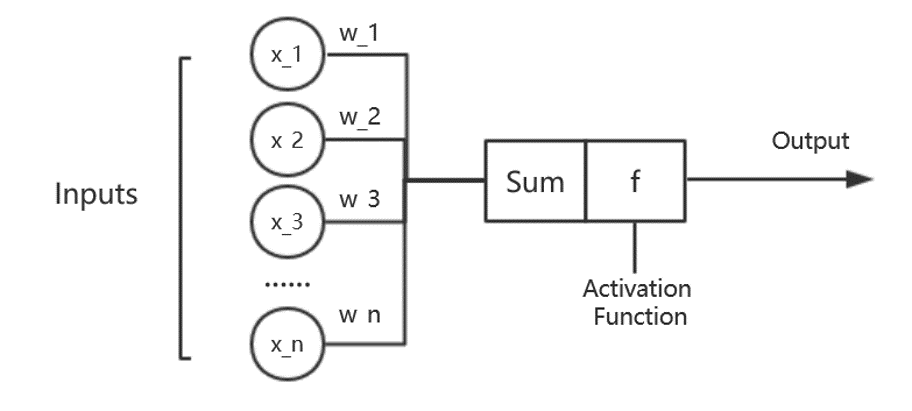
\includegraphics[width=10cm,height=4cm]{Figures/Chapter03/AN.PNG}
\caption{人工神经元结构}
\label{fig3-AN}
\end{center}
\end{figure}


人工神经网络靠的是正向和反向传播来更新神经元,从而形成一个完整的神经系统,本质上,这是一个能让计算机处理和优化的数学模型。而生物神经网络是通过刺激,产生新的联结,让信号能够通过新的联结传递而形成反馈。那么神经元是如何学习事物特征的呢?人工神经元的学习过程被视为一个权重优化不断迭代的结果。也由此也确定这种学习类型是监督学习。权重的调整,以训练数据为基础,结果是已知的类型[也即监督学习]。优化权重是为了最小化损失函数,最优权重可以用来计算未知数据预测结果的类别概率。%这也表明对预期结果的概率。
这里面涉及权重函数的优化和随机梯度算法。从关系上说,就是通过随机梯度下降实现权重优化。

一开始模型只是简单的线性回归模型,作用是为了实现分类。这种类型模型是一个简单神经元的模型,而是线性模型。这样对非线数据的处理就要考虑新的问题。故而引入激活函数(Activate Function)。从另一个侧面考虑了人工神经元会自动学习事物特征,自然而然涉及随机梯度下降算法(或随机梯度上升算法)。下面先介绍简单回归模型Percepton,理解其中的激活函数等,再通过Adaline 理解随机梯度下降算法\ref{fig3-PA}。

\begin{figure}
\begin{center}
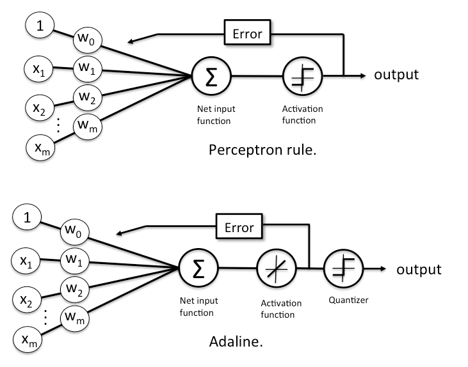
\includegraphics[width=10cm,height=8cm]{Percepton-Adaline.PNG}
\caption{人工神经元模型规则}
\label{fig3-PA}
\end{center}
\end{figure}

在感知机(Percepton)模型中,这里可以看做一个线性回归模型。
对于线性回归问题,优点:结果易于理解,计算上不复杂。缺点:对非线性的数据拟合不好。适用数据类型:数值型和标称型数据。
假设寻找找到最佳拟合直线:y=0.1*x-0.3, 0.1和-0.3 称为回归系数。这样一条直线的确立也是对二分类问题的解。利用线性回归得到最佳拟合曲线,其实求回归方程中的系数,就可以得到回归方程。一般使用的求解方法是最小二乘法。而得到最佳拟合曲线一旦得到,对于新的数据的分类问题,自然而然能够预测该数据属于哪个类别,这也是回归作为分类学习算法的原理。

$X$ =
$\left(
  \begin{array}{ccccc}
    x_{11} & x_{12} & \cdots & x_{1d} & 1 \\
    x_{21} & x_{22} & \cdots & x_{2d} & 1 \\
    \vdots & \vdots & \ddots & \vdots & \vdots \\
    x_{m1} & x_{m2} & \cdots & x_{md} & 1 \\
  \end{array}
\right)
$
=
$\left(
   \begin{array}{cc}
     x^{T}_{1} & 1 \\
     x^{T}_{2} & 1 \\
     \vdots & \vdots \\
     x^{T}_{m} & 1 \\
   \end{array}
 \right)
 $

再把标记也写成向量形式 $\bf{y}$ = ($y_{1}$;$y_{2}$;$\ldots$;$y_{m}$), 则得到的解便是回归系数。

上面的问题是一个线性数据模型,可以认为该模型的传递函数为恒等式(即保持数值不变);直接输出结果。当数据是非线性关系的时候,就考虑新的模型处理数据。引入Logitic 回归。而对Logistic回归而言,传递函数是Sigmoid函数。传递函数即为激活函数。Logitic 回归模型解决非线性二分类问题。那么多分类问题就需要用softmax函数。Softmax分类是对Logistic回归在多个不同的值上的推广。 Logistic回归的激活函数是 Sigmoid函数,而Softmax的激活函数是 一个叠加的Sigmoid函数。
\begin{figure}[htbp]
\begin{center}
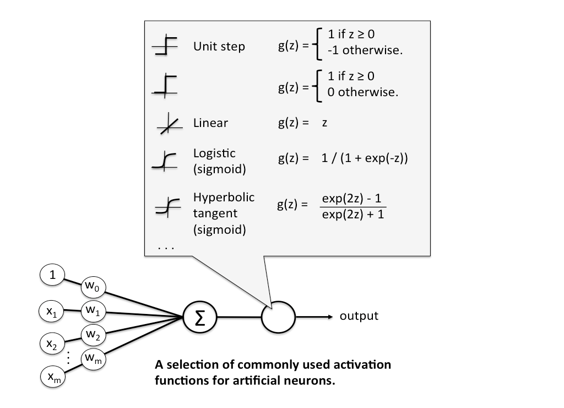
\includegraphics[width=12cm,height=10cm]{AFunction.PNG}
\caption{激活函数}
\label{fig3-AF}
\end{center}
\end{figure}

那么权重函数是如何优化?$W $代表特征权重(Weight),首先给一个随机初始值(可以相等,也可以考虑用截断的高斯分布随机值)。这里假定对数据建模的公式为$y_i = W_i*X_i + bias_i$,bias作为偏差值(也是阈值)决定最后y的分类结果。如果模型的学习结果跟实际结果相同,则这个权重是非负比例的特征权重,所以不对权重进行调整,但是如果模型的学习结果与实际结果相反,则这一次学习对权重需要有所调整。推导如\ref{eq3-weight}所示。

\begin{align}
 W     &:=\  W\ +\ \Delta W     \label{eq3-weight}  \\
 \Delta W_j &=\  -\eta \frac{\partial J}{\partial W_j}\ \nonumber \\
 &=\  \ -\eta \sum_i (target^{(i)} - output^{(i)})(-x_j^{(i)})  \nonumber     \\
 &=\  \eta \sum_i (target^{(i)} - output^{(i)})x_j^{(i)}
\end{align}
其中 $J$是目标函数(成本函数),也是用来判别结果是否来调整权重的损失函数。$\eta$是学习率,一般学习率设置需要适当,不然会导致取不到最优值,也可能会陷入局部最优值。
\begin{align}
  \frac{\partial J}{\partial W_j} &=\  \frac{\partial}{\partial W_j} \sum_i \frac{1}{2} (target^{(i)} - output^{(i)})^2\ \nonumber \\
 &=\    \frac{1}{2}  \sum_i \frac{\partial}{\partial W_j} (target^{(i)} - output^{(i)})^2   \nonumber     \\
 &=\  \frac{1}{2}  \sum_i 2 * (target^{(i)} - output^{(i)})\frac{\partial}{\partial W_j} (target^{(i)} - output^{(i)}) \nonumber \\
 &=\   \sum_i  (target^{(i)} - output^{(i)})\frac{\partial}{\partial W_j} (target^{(i)} - \sum_j w_j x_j^{(i)})  \nonumber \\
 &=\   \sum_i (target^{(i)} - output^{(i)})(-x_j^{(i)})
\end{align}

总结来说,人工神经元通过卷积核映射学习数据特征,通过正向或反向传播传递误差,在随机梯度下降算法支持下优化损失函数,从而更新权重函数,进而实现对数据特征自动学习。

\subsection{卷积神经网络}
从提出人工神经元,到提出卷积神经网络。自1998年Lecun等人\cite{lecun2015lenet}实现第一个运算完整的卷积神经网络模型LeNet-5模型,在这之后网络基本结构就相对固定下来了。后续在(Large Scale Visual Recognition Challenge)中提出了更多更复杂有效的模型,按照提交时间排序为AlexNet(2012)\cite{krizhevsky2012imagenet},
VGG-16(2014),
Inception-v1(,
Inception-v3,
ResNet-50(
Xception
Inception-v4
Inception-ResNets
ResNeXt-50(2015)
这些模型都在不同应用比赛中名列前茅。

% definition
卷积神经网络 ( Convolution neural network, CNN ) 由一组非线性函数映射或者仿射变换函数组成,通过学习训练数据,得到由训练集定义的经验分布,从而用来预测未来数据的概率分布函数等等。之所以称为“卷积神经网络”,表明该神经网络中至少一层使用了卷积( convolution ) 运算。卷积网络会提供一些工具,在具体环境中选择相应的工具给出通用的准则很有必要。卷积神经网络结构的研究进展发展很迅速,以至于针对特定基准(benchmark),没多久就会公开一个新的最优的网络结构。

对于一般的二分类问题而言,卷积神经网络通过学习这两个类别数据的不同之处来得到一个“分类器”,在应用这个“分类器”,之后能得到描述两个分布的概率密度函数,我们一般只关心正样本数据的概率分布。

%更细致地来说,从感知机(Perceptron)发展到卷积神经网络,其基本原理是在高维空间中,寻找一个最优的分割面,也被称为边界超平面,这个分割面能将不同类别的数据集分离。但是最开始的“MP"模型或感知机,他们只针对线性可分或近似线性可分的数据集有很好的效果,对于线性不可分的数据,后者渐渐发展激活函数,可以部分解决这种问题。





%\subsection{卷积神经网络结构}
卷积神经网络一般是针对图像处理,其特点表现在卷积层的作用,卷积层类似于自动提取信号特征,再借助激活函数做降维或者分类。一般的卷积神经网络有以下四层,第一是输入层,处理数据格式;第二是卷积层,自动提取特征;第三是池化层,降低数据维度,提取更高代表性特征,第四是全连接层(类似多层感知机),输出结果。这种结构下一定会卷积层,中间的隐层层的构建取决于数据构建与结果分析。

\begin{figure}[htbp]
\begin{center}
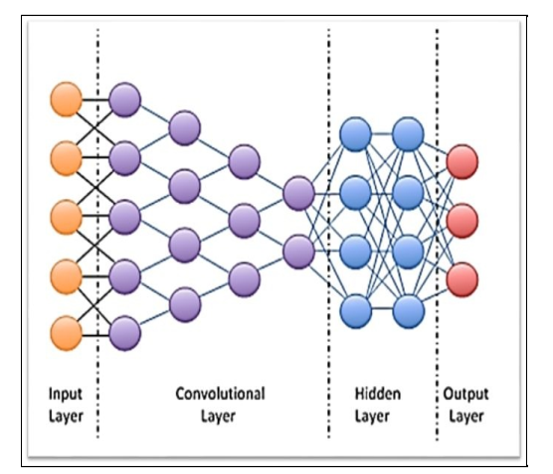
\includegraphics[width=8cm,height=5cm]{CNN.PNG}
\caption{CNN结构;图片来自\cite{zaccone2018deep}}
\label{fig3-CNN}
\end{center}
\end{figure}

所以一般卷积神经网络的层次结构分为:输入层-卷积层-激励层-池化层-(迭代)-全连接层-输出层。下面分层功能进行解释。

%\subsubsection{卷积层}
卷积层一般用于自动提取特征,其中卷积运算是理论上是对两个实变函数的一种数学运算(operation)。在一些数据上,比如时间序列函数,时间上越近的测量结果越相关。故而会采取某种运算使得对最近的测量结果赋予更高的权重,例如采用加权平均操作。实现这种运算可以得到卷积的定义。卷积运算通常用"*"表示。
$$s(t)=(x*w)(t)$$

一般而言,卷积的第一个参数(即公式中的“x”)通常是输入(input),第二个参数(函数“w”)叫做核函数(kernel function)。输出一般被称作特征映射(feature map)。
具体举例来说,
假设输入的图像数据为5*5=25的图像;卷积核为3*3=9的矩阵,那么移动卷积核过程中提取出来的特征是3*3=9的特征矩阵。
\begin{figure}[htbp]
\begin{center}
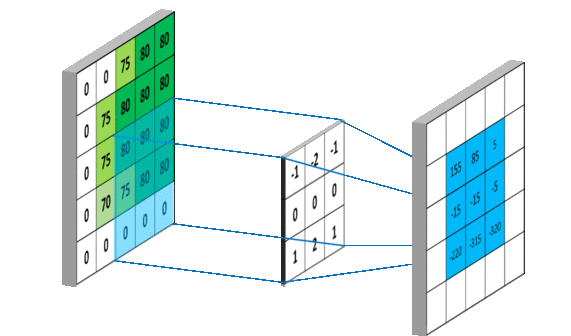
\includegraphics[width=12cm,height=6cm]{cl.PNG}
\caption{卷积层;图片来自\cite{Robinson2018}}
\label{fig3-CL}
\end{center}
\end{figure}

在机器学习应用中,输入通常是多维数据,而核函数是由学习算法优化得到多维数组的参数。卷积运算不仅仅可以在一个维度上做运算,也可以多维做运算,而且可以实现可交换。

%卷积层实现自动提取特征功能。
实际训练过程中,
每层卷积层由若干卷积单元组成,每个卷积单元的参数都是通过反向传播算法优化。卷积运算的目的是提取输入数据的不同特征,第一层卷集层可能只能提取一些低级的特征,如边缘、线条、和角等层级,更高层的网络是从底层的特征中迭代提取出来的,称为更加复杂的特征。
    %在卷积层中提取特征我们需要用到卷积核,卷积核就是一个矩阵。

%\subsubsection{池化层}
%池化层实现特征的表示与降维。
池化层,也称为下采样,与之相对的是上采样(卷积层),主要用于特征降维,压缩或减少数据和参数的数量,减少过拟合,同时提高模型的容错性和训练速度。池化层的输入一般源于上一个卷集层的输出,它的作用是保留主要的特征,同时减少下一层的参数和计算量,防止过拟合。如保持某种不变性,平移、选旋转、尺度缩放、加噪声等等。

 \begin{figure}[htbp]
\begin{center}
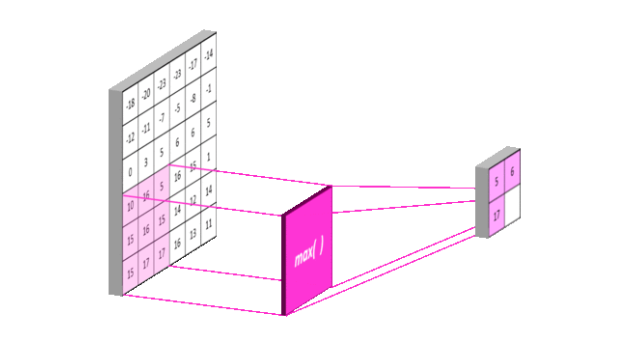
\includegraphics[width=12cm,height=6cm]{pl_2.PNG}
\caption{池化层;图片来自\cite{Robinson2018}}
\label{fig3-PL}
\end{center}
\end{figure}
一般采用的方法有最大池化和均值池化。(最大值采样、均值采样)选择最大池化层和平均池化层的区别。最大池化层是提取最明显的特征,平均池化 层是顾及每一个像素,取平均值。
 \begin{figure}[htbp]
\begin{center}
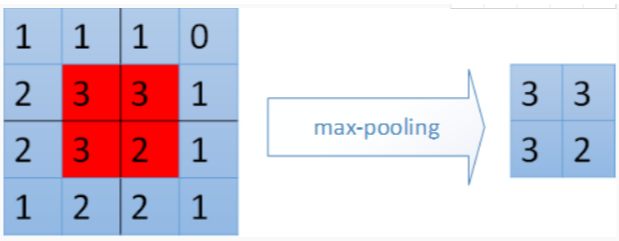
\includegraphics[width=8cm,height=4cm]{maxSampling.PNG}
\caption{最大池化:图片来自\cite{Robinson2018}}
\label{fig3-MS}
\end{center}
\end{figure}
 \begin{figure}[htbp]
\begin{center}
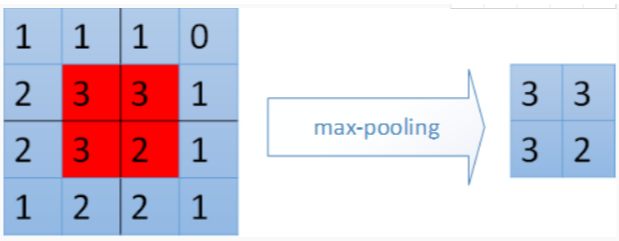
\includegraphics[width=8cm,height=4cm]{maxSampling.PNG}
\caption{均值池化;图片来自\cite{Robinson2018}}
\label{fig3-MaxS}
\end{center}
\end{figure}

%\subsubsection{全连接层}
全连接层的作用就是类似于多层感知机。把之前通过多层神经元映射得到的特征映射图结合起来,且经过激活函数,多层的神经元激活使得当前最优且线性不可分的特征表示 通过非线性的激活操作,使得数据(以特征表示)在输出层变成线性可分。全连接层一般为两到三层,神经网络的性能就到达一定的极值[黄安埠《深入浅出深度学习(原理剖析与python实践]

%\subsubsection{激活函数}
无论经过卷积成还是池化层,出来的数据都是连续性的,假设数据的范围在0与1之间,那么可以是0和1之间的任何数。线性化的模型不能直接解决类似“异或”这种非线性化的问题。
    
而选取激活函数是用来加入非线性因素的考量,因为线性模型的表达能力不够。对于时间序列,我们也采用的是卷积方式来处理,对每个时间观测值都赋予一个权值,这个操作显然是线性的。但是对于我们的样本来说不一定是线性的,为了解决这个问题,我们可以进行线性变换,或者引入非线性的因素解决问题,即隐藏层中激活函数的引入。非线性的激活函数使得复杂的非线性数据集也能被处理,且切实提高了模型的学习和表示能力。经过激活函数处理后,模型中神经元会被赋予不同权重,权重意味这该神经元是否被激活,那该神经元所表示的数据的特征就会不同程度地被采纳,从而实现模型能自动提取特征的作用。

% 举例说明 激活函数的作用
举例来说,Lee等人在音频的时间序列里,通过时频图来展示一个音频数据,经过激活函数后的特征权重被调整为(0,1)之内的值,且遵循sigmoid函数的特性。不同的权重意味着对不同特征的重视程度,多种特征的组合之后得到最优特征表示,达到关键信息中自动提取关键特征的作用。
\begin{figure}[htb]
 \centering
 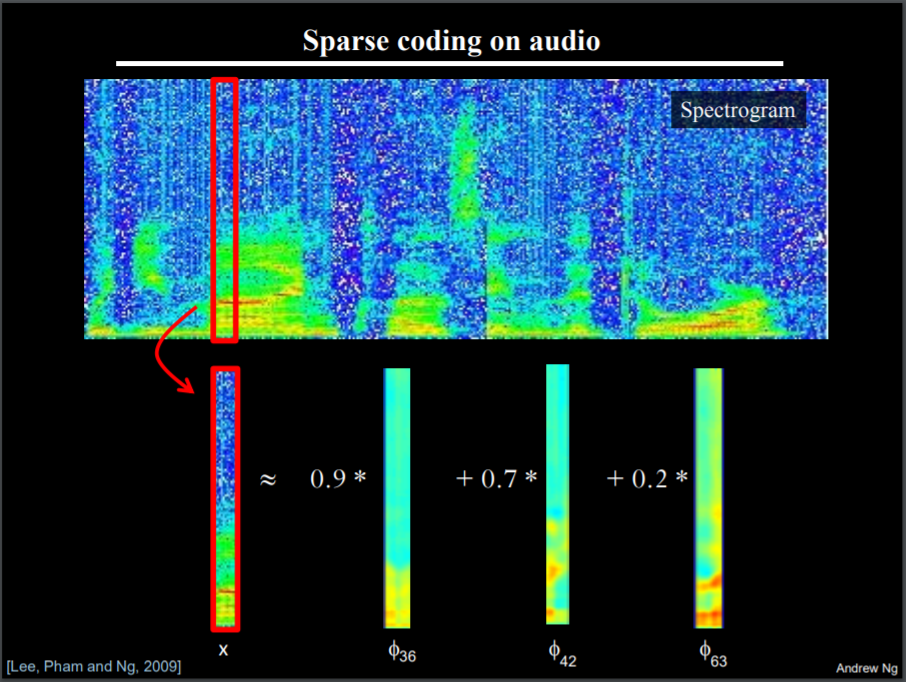
\includegraphics[width=.8\linewidth]{SparseRepresent.png}
    \caption{\label{fig:SR}音频数据时频图的自动提取特征过程}
\end{figure}



在卷积神经网络中,Alex等人\cite{krizhevsky2012imagenet}研究表明Relu函数比传统激活函数(如sigmoid函数)优,能够缓解训练过程中的梯度消失问题。具体表达式如式(\ref{eq3-relu})所示,。
\begin{equation}
ReLU(x)=
\begin{cases}
x& \text{if\ x $>$ 0}\\
0& \text{if x $\leq$ 0}
\end{cases}
\label{eq3-relu}
\end{equation}


\begin{comment}
\subsection{数据集准备}
%\subsubsection{数据集准备}

在机器学习算法中,一般会准备3种数据集,分别是训练数据集、验证数据集和测试数据集。他们三个数据集完全不同,他们的作用也各不相同。训练数据集顾名思义用来训练神经网络算法,使得神经网络算法能够从中学习到数据的特性或特征。而验证数据集则用来检验神经网络学习效果,如果神经网络算法也能够正确辨别验证数据集,证明该算法正走向正确标签的类别,如果不能正确辨识验证数据集,则会用来惩罚该学习过程,使得学习过程能够修正方向。故而训练数据和验证数据一般是独立同分布(Independently Identically Distribution, IID )的数据构成。最后是测试数据集,这个一般是正式应用的数据集打包而成。而且最接近真实应用场景的数据,它一般只经过最少的数据预处理,用于检验前面训练得到的神经网络算法是否具备真实辨识能力和能做到什么样的程度。

在这个过程中,其实假设了真实数据的分布信息蕴含在数据中,但是有时候真实数据量很少,并不能完全分割为三种数据集,且我们并不知道数据真实分部信息。所以采用了模拟的数据集,假设了数据服从更宽泛的分布范围,神经网络算法能从中学习,且能够应该于真实分布的测试数据。故而,我们采用的训练数据要尽可能采用更宽泛的分布模拟数据,用于检验该算法学习效果的验证数据集也采用跟训练数据一样的分布信息。测试数据集采用真实的观测数据或者最接近真实的模拟数据。具体来说,在本论文中,训练数据和验证数据中波形是采用同样随机分布得到所有引力波源参数(如中心黑洞质量都是采用log分布)产生的EMRI波形,而测试数据集则采用天文学模型得到引力波源参数来产生EMRI波形。之后都是以同样方式叠加模拟的高斯噪声,用来作为正样本。在三种数据集中的负样本都是同样方法产生的随机高斯噪声。
\end{comment}

\subsection{循环神经网络}
%\subsubsection{循环神经网络}
循环神经网络(Recurrent Neural Network,RNN)是一类专门用于处理时序数据样本的神经网络,它的每一层不仅输出给下一层,同时还输出一个隐状态,给当前层在处理下一个样本时使用。就像卷积神经网络可以很容易地扩展到具有很大宽度和高度的图像,而且一些卷积神经网络还可以处理不同尺寸的图像,循环神经网络可以扩展到更长的序列数据,而且大多数的循环神经网络可以处理序列长度不同的数据(for 循环,变量长度可变)。它可以看作是带自循环反馈的全连接神经网络。
%其网络结构如下图所示。

\begin{figure}[htbp]
\begin{center}
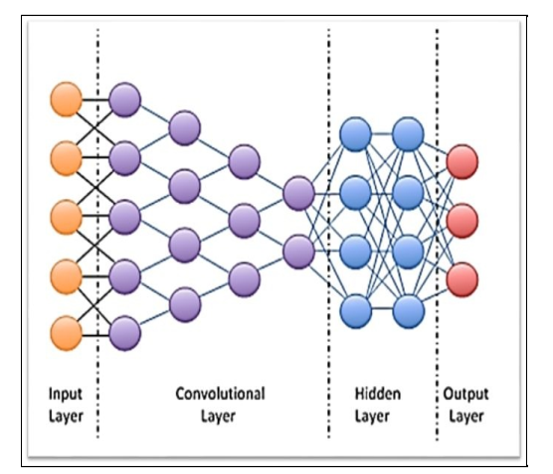
\includegraphics[width=8cm,height=6cm]{CNN.PNG}
\caption{RNN结构;图片来自\cite{zaccone2018deep}}
\label{fig3-RNN}
\end{center}
\end{figure}

长短时记忆网络(LSTM),时序反向传播算法按照时间的逆序将错误信息一步步地往前传递。当每个时序训练数据的长度$T$较大或者时刻$t$较小时,损失函数关于$t$时刻隐藏层变量的梯度比较容易出现消失或爆炸的问题(或称长期依赖问题)。


\begin{comment}
\subsection{探测结果分析}
%描述四种概率
%描述误报率和阈值的计算,比如如何求出来的信噪比大于8
%ROC curve 和efficiency curve

%描述如何计算阈值的过程,这很有分量,但是实际我还没有算出来为什么是20?是由于模板的精度决定的吗?
在信号探测中,检测概率和错误概率是最常需要的计算。目前在我们理论计算过程中,通常假设噪声都是高斯噪声,实际探测过程会是非高斯、非稳态的噪声,但这种需要在实际仪器运行过程中才能评估噪声特性。所以我们还是基于高斯稳态噪声的假设下进行的探测检验。

高斯噪声n(t)顾名思义其数据点特性满足高斯分布,则n分布密度函数为:

$p(n)=\frac{1}{\sqrt{2\pi}\sigma}e^{-(n-\mu_n)^2/2\sigma_n^2}$

公式中$\mu_n$和$\sigma_n^2$分别是噪声的均值和方差。从高斯函数特性也可得到n的累积分布函数(cumulative distribution function, CDF)为:

$F(n)=\int_n^{\infty}p(n)dn = \frac{1}{\sqrt{2\pi}}\sum_n^{\infty}e^{-(n-\mu_n)^2/2\sigma^2_n}
=\frac{1}{2}\frac{2}{\sqrt{\pi}}\sum^{\infty}_{(n-\mu_n)/\sqrt{2}\sigma}{e^{-t^2}dt}$

定义误差函数(error function)
$$
和误差补余函数
$$

则可以把累积分布函数和误差函数以及误差补余函数函数都串联起来。
即高斯噪声n的累积分布函数可以写成:
$F(n)=\frac{1}{2}erfc(\frac{(n-\mu_n)}{\sqrt{2}\sigma_n})=\frac{1}{2}[1-erf(\frac{(n-\mu_n)}{\sqrt{2}\sigma_n})]$

\end{comment}
%\section{参数估计}